% !TeX root = ../main.tex

\section{Automazione del Processo di Sviluppo}

\begin{frame}{Flusso di Lavoro}
    \begin{columns}[onlytextwidth]
        \begin{column}{0.95\textwidth}
            \begin{figure}[H]
                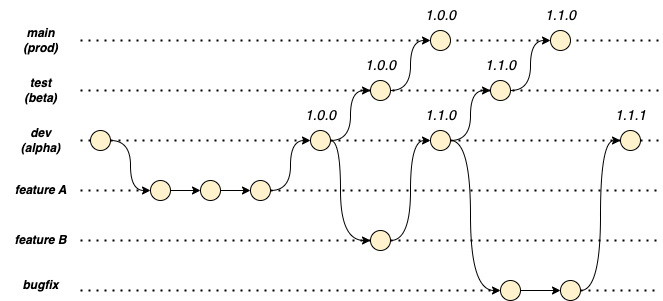
\includegraphics[width=0.9\textwidth]{img/branching-model.png}
            \end{figure}
        \end{column}
        \begin{column}{0.05\textwidth}
        \end{column}
    \end{columns}
    \vspace{5mm}
    \begin{columns}[onlytextwidth]
        \begin{column}{0.4\textwidth}
            \textbf{Branch principali}:
            \begin{itemize}
                \item dev
                \item test
                \item main
            \end{itemize}
        \end{column}
        \begin{column}{0.4\textwidth}
            \textbf{Ambienti}:
            \begin{itemize}
                \item Testing interno (alpha)
                \item Testing esterno (beta)
                \item Produzione (prod)
            \end{itemize}
        \end{column}
    \end{columns}
\end{frame}

\begin{frame}{Continuous Integration/Delivery}
    \vspace{3mm}
    \begin{columns}[onlytextwidth]
        \begin{column}{0.45\textwidth}
            \textbf{Continuous Integration}
            \vspace{2mm}
            \begin{itemize}
                \item \textbf{Principio}: Integrazione frequente di piccole modifiche, testate automaticamente
                \vspace{2mm}
                \item \textbf{Stages}:
                \begin{itemize}
                    \item Build
                    \item Test
                    \item Package
                \end{itemize}
            \end{itemize}
        \end{column}
        \begin{column}{0.45\textwidth}
            \textbf{Continuous Delivery}:
            \vspace{2mm}
            \begin{itemize}
                \item \textbf{Principio}: Rilascio frequente di piccole modifiche o funzionalità, eseguito in modo automatico
                \vspace{2mm}
                \item \textbf{Stages}:
                \begin{itemize}
                    \item Release alpha
                    \item Release beta
                    \item Release prod
                \end{itemize}
            \end{itemize}
        \end{column}
    \end{columns}
    \begin{figure}[H]
        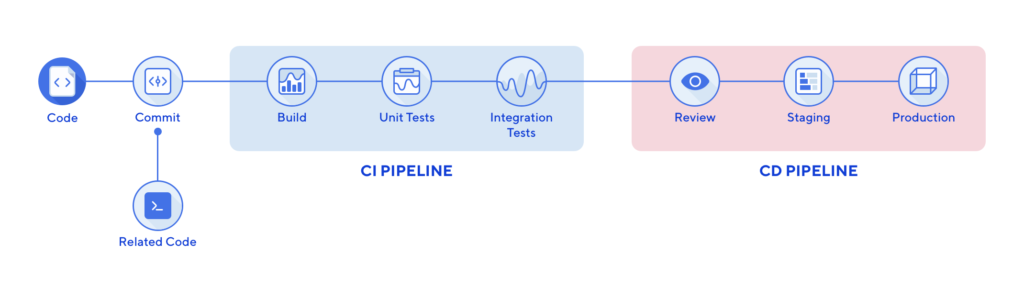
\includegraphics[width=1\textwidth]{img/ci-cd-pipeline.png}
    \end{figure}
\end{frame}

\begin{frame}{Continuous Inspection}
        \begin{columns}[onlytextwidth]
        \begin{column}{0.45\textwidth}
            \textbf{Continuous Inspection}
            \vspace{2mm}
            \begin{itemize}
                \item \textbf{Principio}: Analisi automatica del codice per garantire un certo livello di qualità e di sicurezza
                \vspace{2mm}
                \item \textbf{Stages}:
                \begin{itemize}
                    \item SAST (Static Application Security Testing)
                    \item SCA (Software Composition Analysis)
                \end{itemize}
            \end{itemize}
        \end{column}
        \begin{column}{0.5\textwidth}
            \begin{figure}[H]
                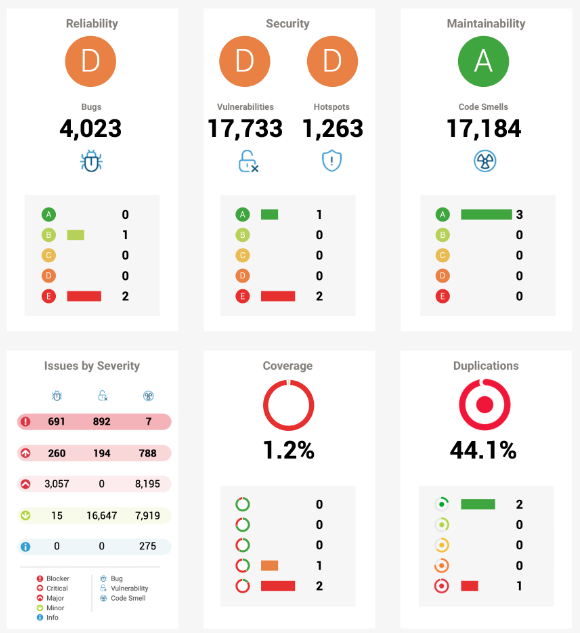
\includegraphics[width=1\textwidth]{img/sonar-screenshot.png}
            \end{figure}
        \end{column}
    \end{columns}
\end{frame}

\begin{frame}{Sistema Obiettivo}
    \begin{figure}[H]
        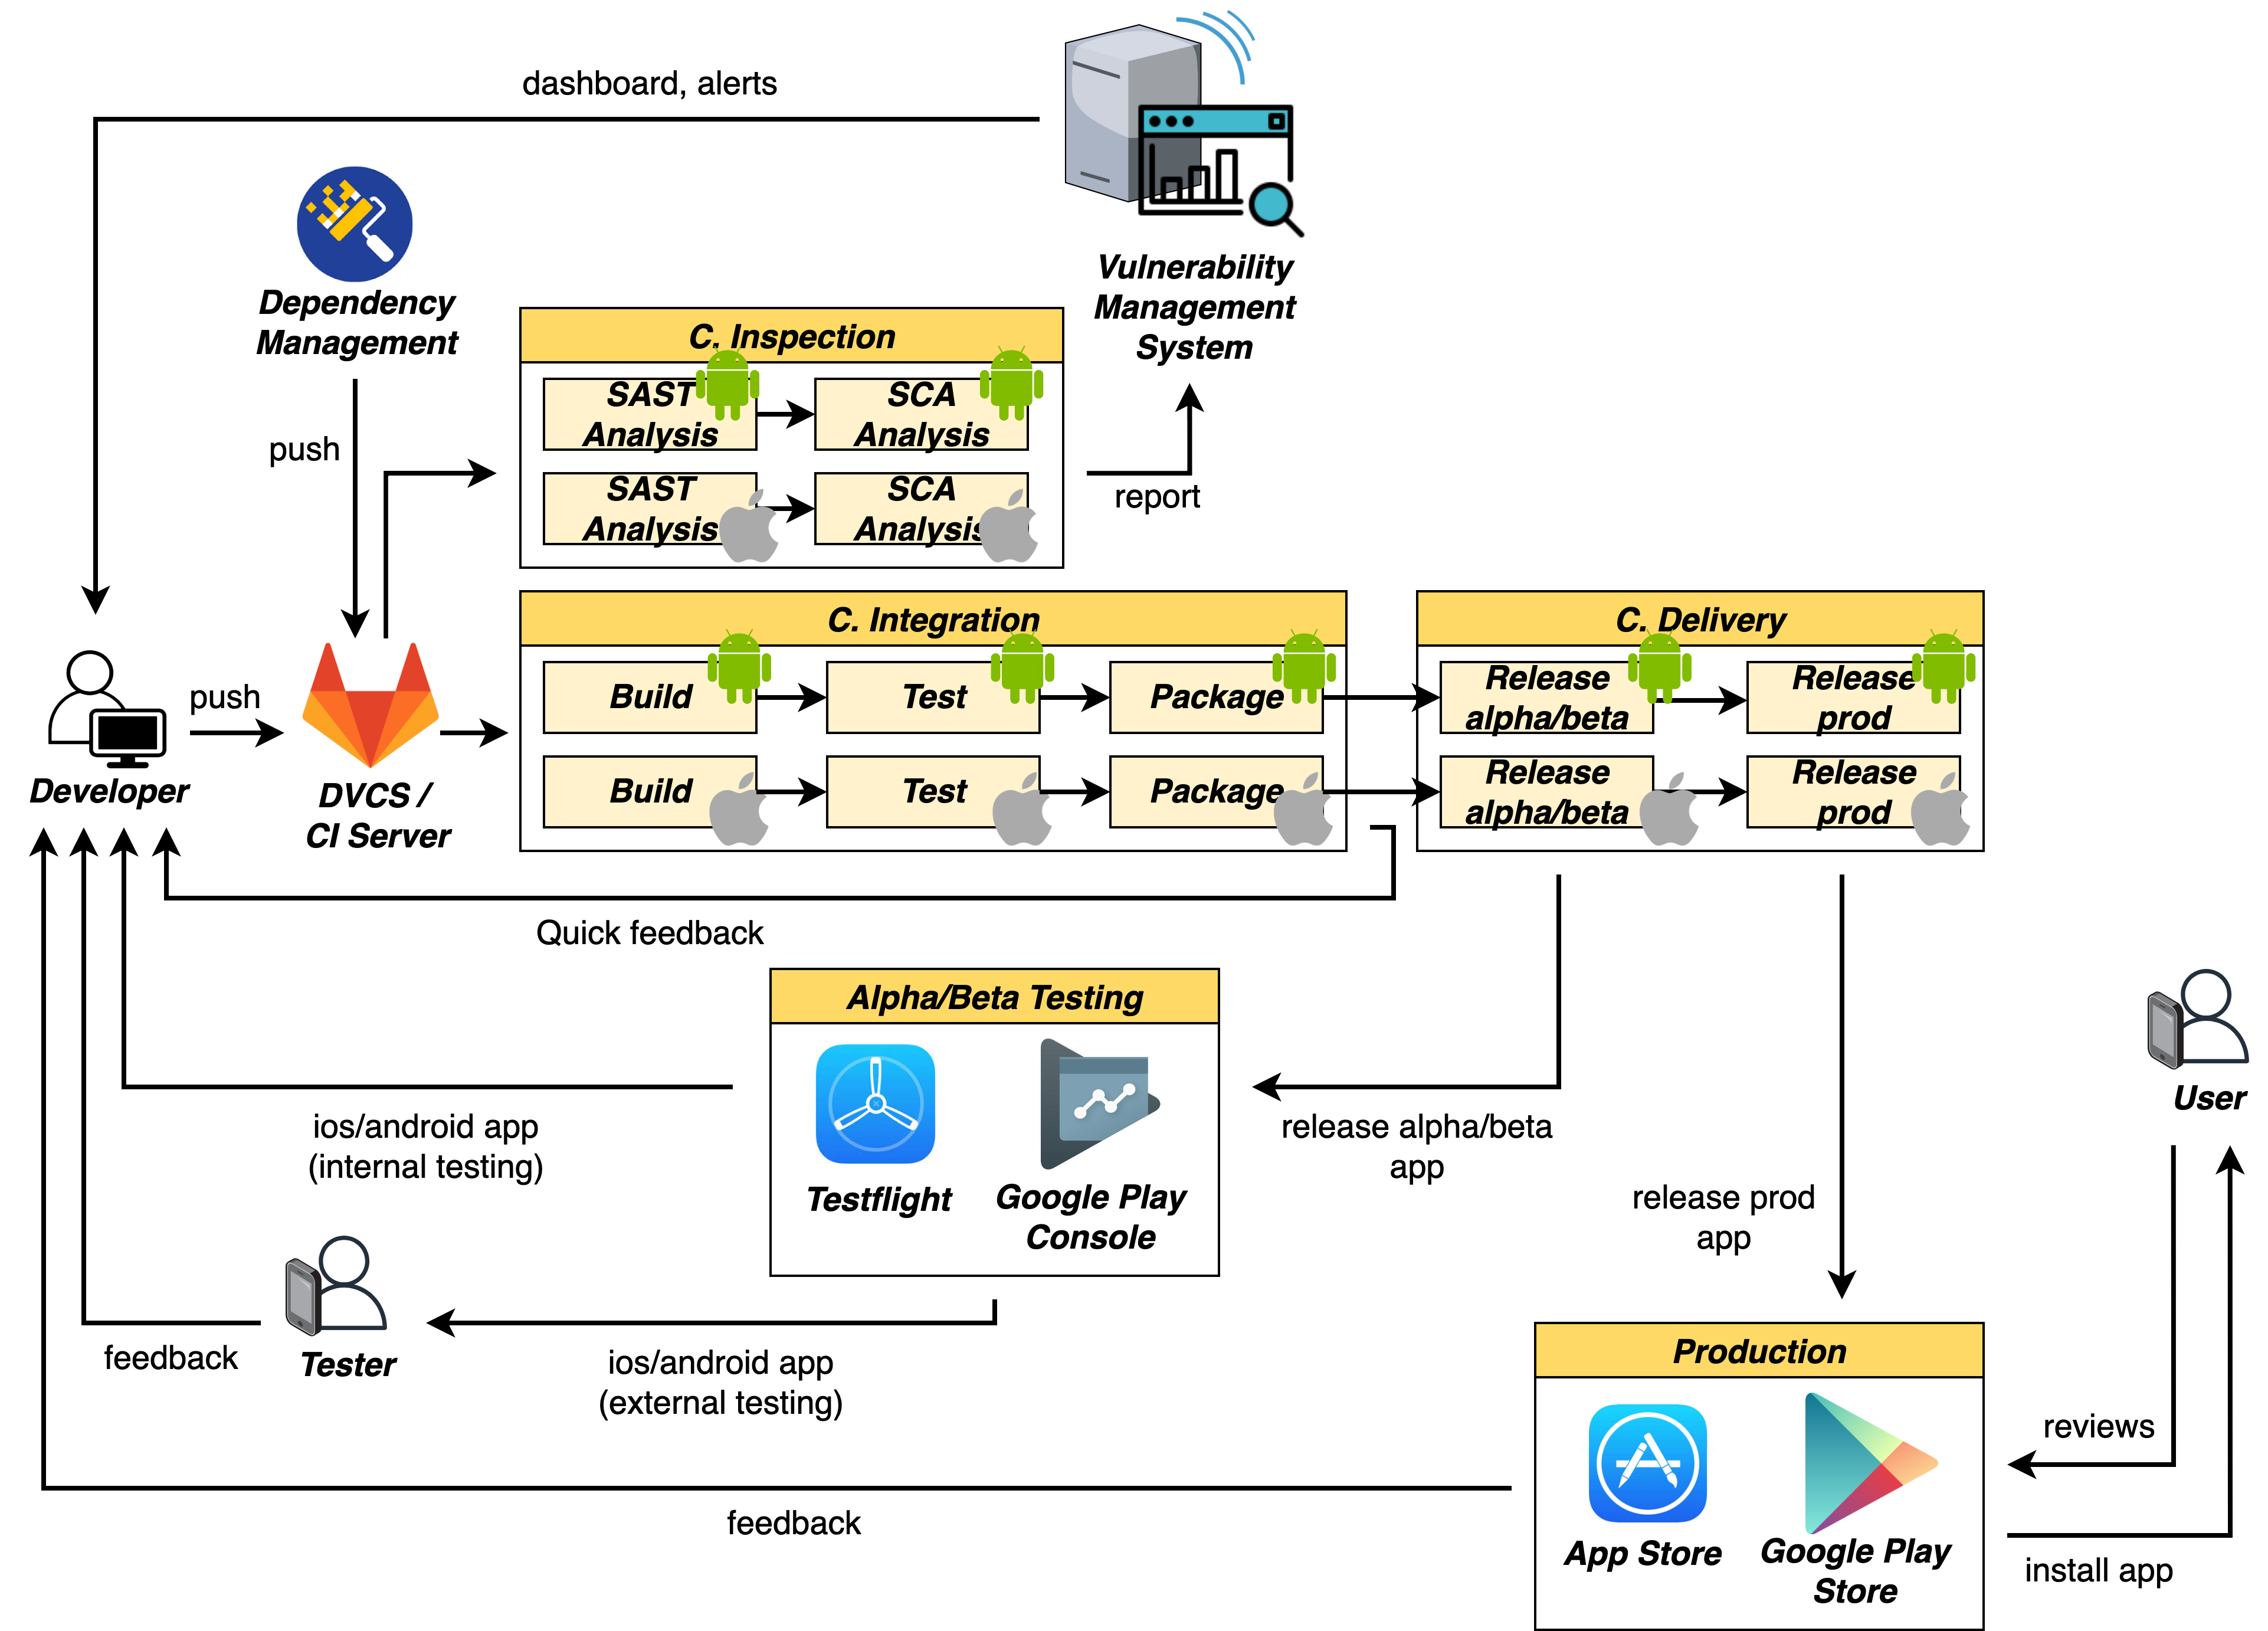
\includegraphics[width=0.89\textwidth]{img/full-cicd.png}
    \end{figure}
\end{frame}